%% Generated by Sphinx.
\def\sphinxdocclass{report}
\documentclass[letterpaper,10pt,english]{sphinxmanual}
\ifdefined\pdfpxdimen
   \let\sphinxpxdimen\pdfpxdimen\else\newdimen\sphinxpxdimen
\fi \sphinxpxdimen=49336sp\relax

\usepackage[margin=1in,marginparwidth=0.5in]{geometry}
\usepackage[utf8]{inputenc}
\ifdefined\DeclareUnicodeCharacter
  \DeclareUnicodeCharacter{00A0}{\nobreakspace}
\fi
\usepackage{cmap}
\usepackage[T1]{fontenc}
\usepackage{amsmath,amssymb,amstext}
\usepackage{babel}
\usepackage{times}
\usepackage[Sonny]{fncychap}
\usepackage{longtable}
\usepackage{sphinx}
\usepackage{graphicx}

\usepackage{multirow}
\usepackage{eqparbox}

% Include hyperref last.
\usepackage{hyperref}
% Fix anchor placement for figures with captions.
\usepackage{hypcap}% it must be loaded after hyperref.
% Set up styles of URL: it should be placed after hyperref.
\urlstyle{same}
\addto\captionsenglish{\renewcommand{\contentsname}{Contents:}}

\addto\captionsenglish{\renewcommand{\figurename}{Fig.\@ }}
\addto\captionsenglish{\renewcommand{\tablename}{Table }}
\addto\captionsenglish{\renewcommand{\literalblockname}{Listing }}

\addto\extrasenglish{\def\pageautorefname{page}}

\setcounter{tocdepth}{1}



\title{cmip5datafinder Documentation}
\author{Valeriu Predoi}
\date{Jul 12, 2017}

\begin{document}

\maketitle

\includegraphics[scale=1.0]{datas}

\section*{Summary}
\phantomsection\label{\detokenize{index:module-cmip5datafinder}}\index{cmip5datafinder (module)}
\begin{itemize}
\item
\textbf{Name:} \sphinxcode{cmip5datafinder.py}
\item
\textbf{Type:} Python script
\item
\textbf{Language:} Python 2.7.13 (Python 2.7+)
\item
\textbf{Synopsis:} Script that searches for data locally (on a mounted disk specified by \sphinxcode{--datasource}) and optionally also on valid ESGF nodes (using \sphinxcode{--synda}). It builds cache files using the results of the search.
\item
\textbf{Needed python modules:} \sphinxcode{sys, os, shutil, getopt, re, string, errno, numpy, subprocess, datetime, time}
\item
\textbf{Developer and contact:} Valeriu Predoi, University of Reading - (\href{valeriu.predoi@ncas.ac.uk}{valeriu.predoi@ncas.ac.uk})
\end{itemize} 

\section*{Introduction and examples}

\sphinxcode{cmip5datafinder.py} is a versatile Python tool that allows building cache files when run on a computer with access to a mounted disk where CMIP5 data is stored under the DRS path system and(or if synda is used) with access to a mounted /sdt/data synda data storage unit and a working synda executable. See below for explanation on synda. It requires minimal input from the user, with most of its functionality coded in as options. Below you can find the command-line options that can be used with the script, see Table \ref{command_line}.

The script uses either a parameter file that contains file parameters on each line or user-specified command-line file parameters.

The script is available to download () and comes prepackaged with an example paramater file (\sphinxcode{example.txt}) to illustrate its functionality and so that the user can run the examples listed below.

\begin{table}[htb!]
\begin{tabular}{ |l|l| }
\hline
\hline
  \sphinxcode{-p, --params-file <file>}    & Namelist file (xml) or text file (txt) or any other input file [REQUIRED] \\ 
                              & e.g. for xml: --params-file ESMValTool/nml/namelist\_myTest.xml \\
                              & e.g. for text: --params-file example.txt \\
                              & e.g. for yaml: --params-file example.yml \\
                              & This option is REQUIRED if --user-input (command line) is NOT present \\
\hline
  \sphinxcode{-h, --help}                  & Display this message and exit \\
\hline
  \sphinxcode{--user-input}                & Flag for user defined CMIP file and variables parameters (to be input at command line \\
                              & with --fileparams for each parameter) \\
                              & This option is REQUIRED if --params-file is not present \\
\hline
  \sphinxcode{--datasource}                & Name of local data source (example: badc). Available datasources: \\
                              & badc [to add more here, depending where running the code][REQUIRED] \\
\hline
  \sphinxcode{--synda}                     & Flag to call synda operations. If not passed, local datasources will be used ONLY \\
\hline
  \sphinxcode{--download}                  & Flag to allow download missing data via synda \\
\hline
  \sphinxcode{--dryrun}                    & Flag to pass if no download is wanted. Don't pass this if downloads are neeeded! \\
                              & If --dryrun in arguments, all cache files will be written as normal but with \\
                              & NOT-YET-INSTALLED flag per file \\
\hline
  \sphinxcode{--fileparams}                & If --user-input is used, this serial option passes one data file argument at a time \\
                              & If --user-input is used, this serial option is REQUIRED \\
                              & e.g. --fileparams CMIP5 --fileparams MPI-ESM-LR --fileparams Amon  --fileparams historical \\
                              & --fileparams r1i1p1 --fileparams 1910 --fileparams 1919 \\
\hline
  \sphinxcode{--uservars}                  & If --user-input is used, this serial option passes one variable argument at a time \\
                              & If --user-input is used, this serial option is REQUIRED \\
                              & e.g. --uservars tro3 \\
\hline
  \sphinxcode{--verbose}                   & Flag to show in-code detailed messages \\    
\hline
\hline
\end{tabular}
\caption{\sphinxcode{cmip5datafinder.py} command-line options.}
\label{command_line}
\end{table}

\paragraph{Example 1: parameter file: workflow description}
(without synda: command:) 

\sphinxcode{python cmip5datafinder.py -p example.txt --verbose --datasource badc}

The code will read each line in \sphinxcode{example.txt}; each line represents a set of file parameters that are parsed (e.g. CMIP5 MPI-ESM-LR Amon historical r1i1p1 1900 1982 tro3); the code will look for relevant files only in the datasource \sphinxcode{badc}, cache the files and output a cache file called \sphinxcode{cache\_example.txt-badc} and a directory called \sphinxcode{cache\_files\_badc}. \sphinxcode{cache\_example.txt-badc} contains rows with four elements: filedescriptor (or header), level of completeness (\sphinxcode{complete} or \sphinxcode{incomplete} or \sphinxcode{missing}), completeness percentage (a \%.2f float) and the available file list. \sphinxcode{cache\_files\_badc} will contain cache files (cache\_cmip5 and missing\_cache\_cmip5) and images describing the file population by model. An example set of images below:

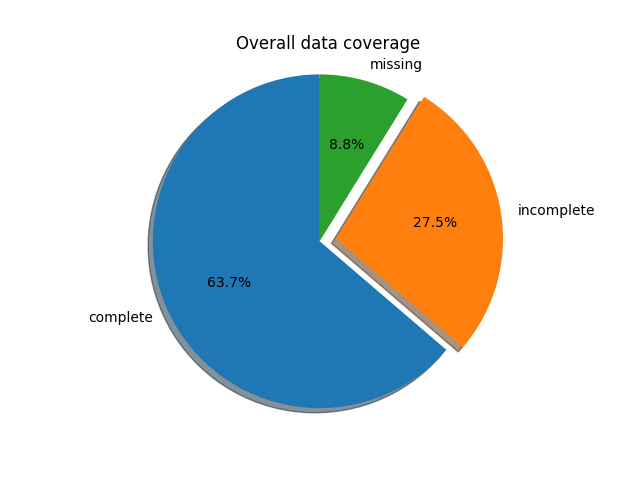
\includegraphics[scale=0.5]{overall}
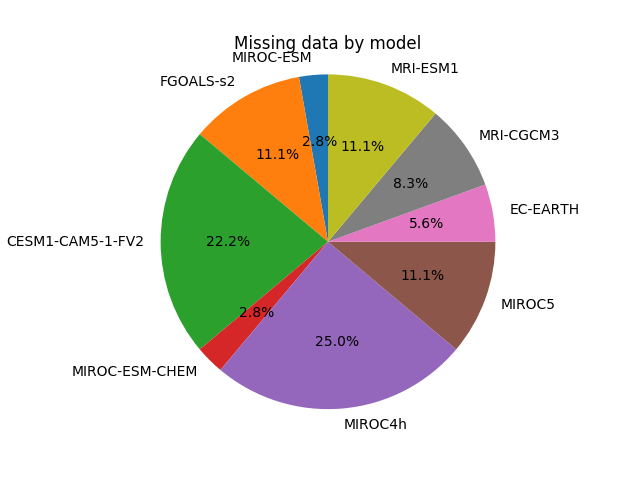
\includegraphics[scale=0.5]{missing}
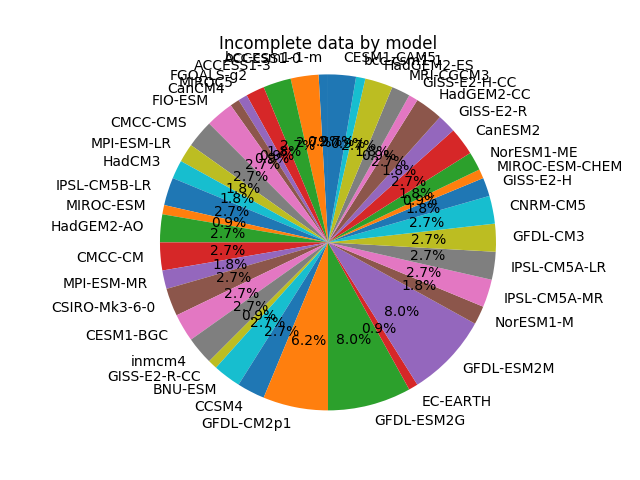
\includegraphics[scale=0.5]{incomplete}

(with synda: command:) 

\sphinxcode{python cmip5datafinder.py -p example.txt --synda --download --dryrun --verbose --datasource badc}

This case builds up on the previous case: the same search is performed within the \sphinxcode{badc} datasource, but the \textbf{missing-only} filedescriptors are searched on ESGF nodes via \textsl{synda} (see \href{https://github.com/Prodiguer/synda}{https://github.com/Prodiguer/synda}). Synda has the capability to complete the incomplete or missing filedescriptors, depending what ESGF servers are listed in its configuration file (we will not discuss this here since that is a system admin issue). Synda will first search in the locally-available locally-mounted \sphinxcode{/sdt/data} disk, and cache whatever is needed and found there, and if (and only if) \sphinxcode{--download} option is specified, synda will go on to search over the remote ESGF servers if files are still needed. \sphinxcode{--download --dryrun} means that synda will search remote ESGF nodes but will not physically download anything found (it will, however, cache it as if it was downloaded but with the field NOT-YET-DOWNLOADED in the cache files for clarity). Synda-only files are stored in caches labelled \sphinxcode{\_synda\_}.


\paragraph{Example 2: command-line args: workflow description}
(with command line args) \sphinxcode{python cmip5datafinder.py --user-input --fileparams CMIP5 --fileparams bcc-csm1-1 --fileparams --fileparams Amon
--fileparams historical --fileparams r1i1p1 --fileparams 1982 --fileparams 2014 --uservars clt --uservars tro3 --uservars pr --datasource badc
--verbose}
Same as above only that the user specifies directly what file they need.

Easy-peasy!

\section*{Main functions}

\index{cache\_merge() (in module cmip5datafinder)}

\begin{fulllineitems}
\phantomsection\label{\detokenize{index:cmip5datafinder.cache_merge}}\pysiglinewithargsret{\sphinxcode{cmip5datafinder.}\sphinxbfcode{cache\_merge}}{\emph{file1}, \emph{file2}, \emph{finalFile}}{}
Function that takes two cache files and merges them
into a single one. Caution -- note the order:
file1 = local datasource cache
file2 = local synda cache

\end{fulllineitems}

\index{date\_handling() (in module cmip5datafinder)}

\begin{fulllineitems}
:0
\phantomsection\label{\detokenize{index:cmip5datafinder.date_handling}}\pysiglinewithargsret{\sphinxcode{cmip5datafinder.}\sphinxbfcode{date\_handling}}{\emph{time1}, \emph{time2}}{}
This function deals with different input date formats e.g.
time1 = 198204 or
time1 = 19820422 or
time1 = 198204220511 etc
More formats can be coded in at this stage.
Returns year 1 and year 2

\end{fulllineitems}

\index{final\_cache() (in module cmip5datafinder)}

\begin{fulllineitems}
\phantomsection\label{\detokenize{index:cmip5datafinder.final_cache}}\pysiglinewithargsret{\sphinxcode{cmip5datafinder.}\sphinxbfcode{final\_cache}}{\emph{parfile}, \emph{ofile1}, \emph{finalfile}}{}
Function that generates the final user-friendly
single cache file; this can easily be used
in various analyses; file legend:
Database \textbar{} data\_status \textbar{} Percent complete \textbar{} available\_data
---------------------------------------------
CMIP5\_MIROC5\_Amon\_historical\_r1i1p1\_2003\_2010\_hus (complete,incomplete or missing) file_list

\end{fulllineitems}

\index{find\_local\_files() (in module cmip5datafinder)}

\begin{fulllineitems}
\phantomsection\label{\detokenize{index:cmip5datafinder.find_local_files}}\pysiglinewithargsret{\sphinxcode{cmip5datafinder.}\sphinxbfcode{find\_local\_files}}{\emph{model}, \emph{out1}, \emph{dirname1}, \emph{mfile}, \emph{latest\_dir}}{}
Function that performs local search for files using {\color{red}\bfseries{}{}`}find'
The depth is as high as possible so that find is fast.
model: CMIP5 MPI-ESM-LR Amon amip r1i1p1
mfile: stderr dump file (cache\_err.out) - need to capture
instances of either Permission denied or non-existent dirs;
latest\_dir: latest version directory e.g. /latest/ on badc
(see above for details)

\end{fulllineitems}

\index{fix\_duplicate\_entries() (in module cmip5datafinder)}

\begin{fulllineitems}
\phantomsection\label{\detokenize{index:cmip5datafinder.fix_duplicate_entries}}\pysiglinewithargsret{\sphinxcode{cmip5datafinder.}\sphinxbfcode{fix\_duplicate\_entries}}{\emph{outfile}}{}
simple fast function to eliminate duplicate entries
from a cache file

\end{fulllineitems}

\index{get\_drs() (in module cmip5datafinder)}

\begin{fulllineitems}
\phantomsection\label{\detokenize{index:cmip5datafinder.get_drs}}\pysiglinewithargsret{\sphinxcode{cmip5datafinder.}\sphinxbfcode{get\_drs}}{\emph{dir1}, \emph{sdir}, \emph{ic}, \emph{model}, \emph{latest\_dir}}{}
Function that returns DRS.
dir1: root directory - /badc/cmip5/data/cmip5/output1/
sdir: subdirectory (institution) - MPI-M
ic: experiment - MPI-ESM-LR
model: CMIP5 MPI-ESM-LR Amon amip r1i1p1
latest\_dir: on badc is /latest/ - this is known in advance
and is dependant on where the code is run.

\end{fulllineitems}

\index{get\_overlap() (in module cmip5datafinder)}

\begin{fulllineitems}
\phantomsection\label{\detokenize{index:cmip5datafinder.get_overlap}}\pysiglinewithargsret{\sphinxcode{cmip5datafinder.}\sphinxbfcode{get\_overlap}}{\emph{tt}, \emph{my1}, \emph{my2}}{}
function that returns the amount of overlap
between needed data and available data
Returns a fractional float
li: list of years from data (1-dim, even number of elements)
my1,my2: required model years

\end{fulllineitems}

\index{lsladir() (in module cmip5datafinder)}

\begin{fulllineitems}
\phantomsection\label{\detokenize{index:cmip5datafinder.lsladir}}\pysiglinewithargsret{\sphinxcode{cmip5datafinder.}\sphinxbfcode{lsladir}}{\emph{dirname}}{}
Calling this function once so we save time; called in root dirname.
It is needed for generalization and not hardcoding the institutions.

\end{fulllineitems}

\index{plotter() (in module cmip5datafinder)}

\begin{fulllineitems}
\phantomsection\label{\detokenize{index:cmip5datafinder.plotter}}\pysiglinewithargsret{\sphinxcode{cmip5datafinder.}\sphinxbfcode{plotter}}{\emph{cachefile}, \emph{saveDir}}{}
simple pie chart plotting function

\end{fulllineitems}

\index{print\_final\_stats() (in module cmip5datafinder)}

\begin{fulllineitems}
\phantomsection\label{\detokenize{index:cmip5datafinder.print_final_stats}}\pysiglinewithargsret{\sphinxcode{cmip5datafinder.}\sphinxbfcode{print\_final\_stats}}{\emph{sfile}}{}
print some final stats
To understand the output, by filedescriptor we mean any file indicator
of form e.g. CMIP5\_MIROC5\_Amon\_historical\_r1i1p1\_2003\_2010\_hus that is fully
determined by its parameters; there could be multiple .nc files
covering a single filedescriptor, alas there could be just one.

\end{fulllineitems}

\index{print\_stats() (in module cmip5datafinder)}

\begin{fulllineitems}
\phantomsection\label{\detokenize{index:cmip5datafinder.print_stats}}\pysiglinewithargsret{\sphinxcode{cmip5datafinder.}\sphinxbfcode{print\_stats}}{\emph{outfile1}, \emph{outfile2}}{}
small function to print some stats at the end

\end{fulllineitems}

\index{synda\_check\_dll() (in module cmip5datafinder)}

\begin{fulllineitems}
\phantomsection\label{\detokenize{index:cmip5datafinder.synda_check_dll}}\pysiglinewithargsret{\sphinxcode{cmip5datafinder.}\sphinxbfcode{synda\_check\_dll}}{}{}
Easy checker on current downloads

\end{fulllineitems}

\index{synda\_dll() (in module cmip5datafinder)}

\begin{fulllineitems}
\phantomsection\label{\detokenize{index:cmip5datafinder.synda_dll}}\pysiglinewithargsret{\sphinxcode{cmip5datafinder.}\sphinxbfcode{synda\_dll}}{\emph{searchoutput}, \emph{varname}, \emph{year1\_model}, \emph{year2\_model}, \emph{header}, \emph{D}, \emph{outfile}, \emph{outfile2}, \emph{download=False}, \emph{dryrunOn=False}, \emph{verbose=False}}{}
This function takes the standard search output from synda
and parses it to see if/what files need to be downloaded

The searchoutput argument is a string and is of the form e.g.

new   221.2 MB  cmip5.output1.MPI-M.MPI-ESM-LR.historical.mon.atmos.Amon.r1i1p1.v20120315.tro3\_Amon\_MPI-ESM-LR\_historical\_r1i1p1\_195001-195912.nc
done  132.7 MB  cmip5.output1.MPI-M.MPI-ESM-LR.historical.mon.atmos.Amon.r1i1p1.v20120315.tro3\_Amon\_MPI-ESM-LR\_historical\_r1i1p1\_200001-200512.nc
new   221.2 MB  cmip5.output1.MPI-M.MPI-ESM-LR.historical.mon.atmos.Amon.r1i1p1.v20120315.tro3\_Amon\_MPI-ESM-LR\_historical\_r1i1p1\_185001-185912.nc

ie typical synda file search output. This gets parsed in and analyzed
against the required model file characterstics and files that comply can
be downloaded via synda install. It also takes the year1\_model and year2\_model, for time checks.
It also takes the variable name and the name of a cache file outfile that will be written to disk.
dryrunOn is the switch from a physical download to just polling the esgf node without any download.

varname: variable
D: incomplete filedescriptors: the dictionary that contains the files that are already available locally
year1\_model, year2\_model: needed filedescriptor year1 and 2
header: unique filedescriptor indicator e.g. CMIP5\_CNRM-CM5\_Amon\_historical\_r1i1p1\_2003\_2010\_hus
outfile: cache file
outfile2: missing cache file
download: download (either dryrun or for reals) flag

\end{fulllineitems}

\index{synda\_search() (in module cmip5datafinder)}

\begin{fulllineitems}
\phantomsection\label{\detokenize{index:cmip5datafinder.synda_search}}\pysiglinewithargsret{\sphinxcode{cmip5datafinder.}\sphinxbfcode{synda\_search}}{\emph{model\_data}, \emph{varname}}{}
This function performs the search for files in synda-standard paths
It takes exactly two arguments:
- a model data string of type e.g. `CMIP5 MPI-ESM-LR Amon amip r1i1p1'
- a variable name as string e.g. `tro3'
It performs the search for files associated with these parameters and returns ALL
available files. (command example: synda search -f CMIP5 MPI-ESM-LR Amon amip r1i1p1 tro3)

\end{fulllineitems}

\index{time\_handling() (in module cmip5datafinder)}

\begin{fulllineitems}
\phantomsection\label{\detokenize{index:cmip5datafinder.time_handling}}\pysiglinewithargsret{\sphinxcode{cmip5datafinder.}\sphinxbfcode{time\_handling}}{\emph{year1}, \emph{year1\_model}, \emph{year2}, \emph{year2\_model}}{}
This function is responsible for finding the correct
files for the needed timespan:

year1 - the start year in files
year1\_model - the needed start year of data
year2 - the last year in files
year2\_model - the needed last year of data
WARNINGS:
we reduce our analysis only to years

\end{fulllineitems}

\index{which\_synda() (in module cmip5datafinder)}

\begin{fulllineitems}
\phantomsection\label{\detokenize{index:cmip5datafinder.which_synda}}\pysiglinewithargsret{\sphinxcode{cmip5datafinder.}\sphinxbfcode{which\_synda}}{\emph{synda}}{}
This function returns the path to the synda exec
or aborts the whole program if synda needs to be used
but its executable is not found.

\end{fulllineitems}

\index{write\_cache\_direct() (in module cmip5datafinder)}

\begin{fulllineitems}
\phantomsection\label{\detokenize{index:cmip5datafinder.write_cache_direct}}\pysiglinewithargsret{\sphinxcode{cmip5datafinder.}\sphinxbfcode{write\_cache\_direct}}{\emph{params\_file}, \emph{ldir}, \emph{rdir}, \emph{outfile}, \emph{outfile2}, \emph{errfile}, \emph{ld}, \emph{verbose=False}}{}
Function that does direct parsing of available datasource files and establishes
the paths to the needed files; makes use of find\_local\_files()
File versioning is controlled by finding the ld = e.g. /latest/ dir
in the badc datasource, this may differ on other clusters and should be correctly
hardcoded in the code!

\end{fulllineitems}

\index{write\_cache\_via\_synda() (in module cmip5datafinder)}

\begin{fulllineitems}
\phantomsection\label{\detokenize{index:cmip5datafinder.write_cache_via_synda}}\pysiglinewithargsret{\sphinxcode{cmip5datafinder.}\sphinxbfcode{write\_cache\_via\_synda}}{\emph{searchoutput}, \emph{varname}, \emph{year1\_model}, \emph{year2\_model}, \emph{header}, \emph{outfile}, \emph{outfile2}}{}
WARNING1: this function is SLOW
WARNING2: this function is not currently used
----------------------------------------------
This function takes the standard search output from synda (synda\_search())
and parses it to see if/what files exist locally

The searchoutput argument is a string and is of the form e.g.

new   221.2 MB  cmip5.output1.MPI-M.MPI-ESM-LR.historical.mon.atmos.Amon.r1i1p1.v20120315.tro3\_Amon\_MPI-ESM-LR\_historical\_r1i1p1\_195001-195912.nc
done  132.7 MB  cmip5.output1.MPI-M.MPI-ESM-LR.historical.mon.atmos.Amon.r1i1p1.v20120315.tro3\_Amon\_MPI-ESM-LR\_historical\_r1i1p1\_200001-200512.nc
new   221.2 MB  cmip5.output1.MPI-M.MPI-ESM-LR.historical.mon.atmos.Amon.r1i1p1.v20120315.tro3\_Amon\_MPI-ESM-LR\_historical\_r1i1p1\_185001-185912.nc

ie typical synda file search output. This gets parsed in and analyzed
against the required model file characterstics and files that comply and
exist locally are stored in a cache file for data reading. It also takes the year1\_model and year2\_model, for time checks.
It also takes the variable name and the name of a cache file outfile that will be written to disk.

\end{fulllineitems}

\end{document}
